\let\negmedspace\undefined
\let\negthickspace\undefined
\documentclass[journal]{IEEEtran}
\usepackage[a5paper, margin=10mm, onecolumn]{geometry}
\usepackage{tfrupee}

\setlength{\headheight}{1cm}
\setlength{\headsep}{0mm}

\usepackage{gvv-book}
\usepackage{gvv}
\usepackage{cite}
\usepackage{amsmath,amssymb,amsfonts,amsthm}
\usepackage{algorithmic}
\usepackage{graphicx}
\usepackage{textcomp}
\usepackage{xcolor}
\usepackage{txfonts}
\usepackage{listings}
\usepackage{enumitem}
\usepackage{mathtools}
\usepackage{gensymb}
\usepackage{comment}
\usepackage[breaklinks=true]{hyperref}
\usepackage{tkz-euclide} 
\usepackage{listings}
\def\inputGnumericTable{}                                 
\usepackage[latin1]{inputenc}                                
\usepackage{color}                                            
\usepackage{array}                                            
\usepackage{longtable}                                       
\usepackage{calc}                                             
\usepackage{multirow}                                         
\usepackage{hhline}                                           
\usepackage{ifthen}                                           
\usepackage{lscape}
\begin{document}

\bibliographystyle{IEEEtran}
\vspace{3cm}

\title{9.2.33}
\author{EE25BTECH11065 - Yoshita J}
{\let\newpage\relax\maketitle}

\renewcommand{\thefigure}{\theenumi}
\renewcommand{\thetable}{\theenumi}
\setlength{\intextsep}{10pt}

\textbf{Question}\\
Find the area of the region enclosed by the parabola \(x^{2}=y\) and the line \(y=x+2\), using the matrix formulation of conics and the intersection-of-line-with-conic formula.\\

\textbf{Solution}:\\

The given ellipse can be expressed as conics with parameters,
\begin{align*}
\vec{x}^{\top}\vec{V}\vec{x}+2\vec{u}^{\top}\vec{x}+f=0,\qquad 
\vec{x}=\myvec{x\\y}.
\end{align*}
where,
\begin{align}
\vec{V}=\myvec{1 & 0\\0 & 0},\qquad
\vec{u}=\myvec{0\\-\tfrac{1}{2}},\qquad
f=0.
\end{align}

The line parameters are 
\begin{align*}
\vec{x}=\vec{h}+\kappa\,\vec{m},\ \kappa\in\mathbb R.
\end{align*}
where,
\begin{align}
\vec{h}=\myvec{0\\2},\qquad \vec{m}=\myvec{1\\1}.
\end{align}

Substituting the given parameters to find the intersection point,
\begin{align}
\kappa=\frac{1}{\vec{m}^{\top}\vec{V}\vec{m}}\Big(
-\,\vec{m}^{\top}(\vec{Vh}+\vec{u})
\pm
\sqrt{\big(\vec{m}^{\top}(\vec{Vh}+\vec{u})\big)^{2}
-\,g(\vec{h})\;(\vec{m}^{\top}\vec{V}\vec{m})}
\Big),
\end{align}
where 
\begin{align}
g(\vec{h})=\vec{h}^{\top}\vec{V}\vec{h}+2\vec{u}^{\top}\vec{h}+f.
\end{align}

Solving,
\begin{align}
\vec{m}^{\top}\vec{V}\vec{m}
=\myvec{1 & 1}\myvec{1 & 0\\0 & 0}\myvec{1\\1}
=\myvec{1 & 1}\myvec{1\\0}=1.
\end{align}

\begin{align}
\vec{Vh}+\vec{u}
=\myvec{1 & 0\\0 & 0}\myvec{0\\2}
+\myvec{0\\-\tfrac{1}{2}}
=\myvec{0\\-\tfrac{1}{2}}.
\end{align}

\begin{align}
\vec{m}^{\top}(\vec{Vh}+\vec{u})
=\myvec{1 & 1}\myvec{0\\-\tfrac{1}{2}}=-\tfrac{1}{2}.
\end{align}

\begin{align}
g(\vec{h})
=\vec{h}^{\top}\vec{V}\vec{h}+2\vec{u}^{\top}\vec{h}
=0+2\myvec{0 & -\tfrac{1}{2}}\myvec{0\\2}=-2.
\end{align}

Now the discriminant,
\begin{align}
\big(\vec{m}^{\top}(\vec{Vh}+\vec{u})\big)^{2}
-\,g(\vec{h})\,(\vec{m}^{\top}\vec{V}\vec{m})
=\left(-\tfrac{1}{2}\right)^{2}-(-2)\cdot 1
=\tfrac{1}{4}+2=\tfrac{9}{4},
\end{align}
so 
\begin{align}
\sqrt{\cdot}=\tfrac{3}{2}.
\end{align}

Hence
\begin{align}
\kappa=\; -(-\tfrac{1}{2})\pm \tfrac{3}{2}
=\tfrac{1}{2}\pm \tfrac{3}{2}\quad\Longrightarrow\quad
\kappa_{1}=2,\ \kappa_{2}=-1.
\end{align}

Points of intersection,
\begin{align}
\vec{x}_{i}=\vec{h}+\kappa_{i}\vec{m}
\end{align}
\begin{align}
\vec{x}_{1}=\myvec{0\\2}+2\myvec{1\\1}=\myvec{2\\4},\qquad
\vec{x}_{2}=\myvec{0\\2}-1\myvec{1\\1}=\myvec{-1\\1}.
\end{align}

Thus the intersection points are 
\begin{align}
\myvec{-1\\1} \quad \text{and} \quad \myvec{2\\4}.
\end{align}

Area of the enclosed region,
\begin{align}
A=\int_{-1}^{2}\big[(x+2)-x^{2}\big]\,dx
=\frac{9}{2}.
\end{align}

Therefore the area of the region enclosed by \(x^2=y\) and \(y=x+2\) is
\begin{align*}
\boxed{\tfrac{9}{2}}
\end{align*}
\begin{figure}[H]
\begin{center}
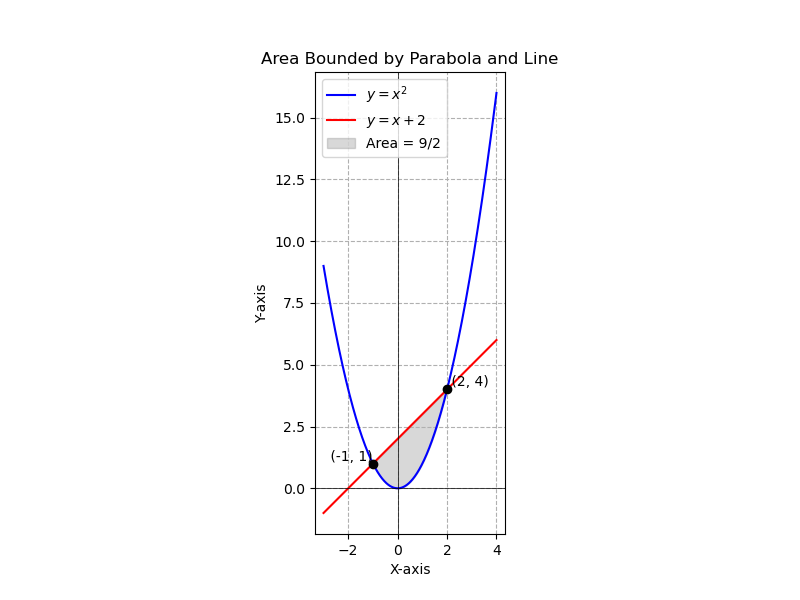
\includegraphics[width=0.9\columnwidth]{figs/fig2.png}
\end{center}
\caption{A plane passing through point A with normal vector n.}
\label{fig:Fig.1}
\end{figure}
\end{document}

